
\section{Trigonometria no Triângulo Retângulo}
\begin{frame} \frametitle{Definição}
\begin{definicao}
Em um triângulo retânglulo $ABC$ como na figura abaixo, define-se o
\sub{cosseno} ($\cos$) e o \sub{seno} ($\sen$) dos ângulos agudos do
triângulo:
\begin{center}
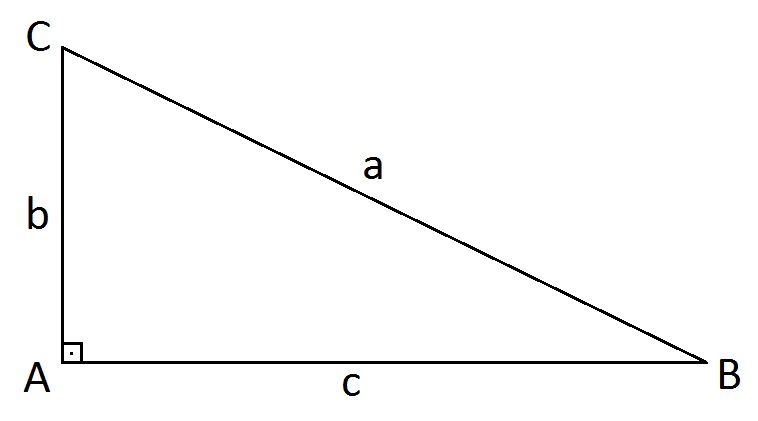
\includegraphics[width=4.8cm]{figures/triangret.jpg}
\end{center}
$$\cos \widehat B = \frac c a = \frac {\text{cateto
adjacente}}{hipotenusa}, \ \ \ \ \sen \widehat B = \frac b a = \frac
{\text{cateto oposto}}{hipotenusa},$$
$$\cos \widehat C = \frac b a \ \ \ \ \text{e} \ \ \ \ \sen \widehat
C = \frac c a.$$
\end{definicao}



\end{frame}

%------------------------------------------------------------------------------------------------------------

\begin{frame}
\frametitle{Propriedades} 
As relações definidas dessa maneira são únicas para cada ângulo em
decorrência da proporcionalidade dos lados de triângulos
semelhantes. Portanto, calcula-se o seno e o cosseno de um ângulo
independentemente do triângulo retângulo que o contém.

\begin{proposicao}
\begin{itemize}
	\item O cosseno de um ângulo agudo é igual ao seno do seu
	complementar e vice-versa. Daí a palavra "cosseno" (seno do
	complemento);
	\item O seno e o cosseno são números compreendidos entre 0 e 1 por
	serem razões entre um cateto pela hipotenusa de um triângulo
	retângulo.
\end{itemize}
\end{proposicao}




\end{frame}

%------------------------------------------------------------------------------------------------------------

\begin{frame}
\frametitle{Senos e Cossenos de Ângulos Notáveis} 

\begin{definicao}
	Os ângulos de $30^\circ$, $45^\circ$ e $60^\circ$ são chamados de  \sub{ângulos notáveis}.
\end{definicao}

\begin{exemplo}
	Os valores do seno e cosseno dos ângulos notáveis são dados na tabela abaixo:
	\begin{center}
		\begin{tabular}{r | c c c}
				& $30^\circ$ & $45^\circ$ & $60^\circ$ \\
		\hline
		$\sen$  & $\dfrac 1 2$ & $\dfrac {\sqrt 2} 2$ & $\dfrac {\sqrt 3} 2$   \\
		$\cos$  & $\dfrac {\sqrt 3} 2$ & $\dfrac {\sqrt 2} 2$ &  $\dfrac 1 2$  		
		\end{tabular}
	\end{center}
\end{exemplo}


\end{frame}

%------------------------------------------------------------------------------------------------------------

\begin{frame}
\frametitle{Relação Fundamental da Trigonometria} 

\begin{proposicao}[Relação Fundamental da Trigonometria]
Seja $\widehat B$ um dos ângulos agudos de um triângulo retângulo
cuja hipotenusa mede $a$ e os catetos, $b$ e $c$. Então:
$$\sen^2 \widehat B + \cos^2 \widehat B = 1.$$
\end{proposicao}
\end{frame}

%------------------------------------------------------------------------------------------------------------